%%%%%%%%%%%%%%%%%%%%%%%%%%%%%%%%%%%%%%%%%
% Beamer Presentation
% LaTeX Template
% Version 1.0 (10/11/12)
%
% This template has been downloaded from:
% http://www.LaTeXTemplates.com
%
% License:
% CC BY-NC-SA 3.0 (http://creativecommons.org/licenses/by-nc-sa/3.0/)
%
%%%%%%%%%%%%%%%%%%%%%%%%%%%%%%%%%%%%%%%%%

%----------------------------------------------------------------------------------------
%	PACKAGES AND THEMES
%----------------------------------------------------------------------------------------

\documentclass{beamer}

\mode<presentation> {

% The Beamer class comes with a number of default slide themes
% which change the colors and layouts of slides. Below this is a list
% of all the themes, uncomment each in turn to see what they look like.

%\usetheme{default}
\usetheme[progressbar=frametitle]{metropolis}
%\usetheme{AnnArbor}
%\usetheme{Antibes}
%\usetheme{Bergen}
%\usetheme{Berkeley}
%\usetheme{Berlin}
%\usetheme{Boadilla}
%\usetheme{CambridgeUS}
%\usetheme{Copenhagen}
%\usetheme{Darmstadt}
%\usetheme{Dresden}
%\usetheme{Frankfurt}
%\usetheme{Goettingen}
%\usetheme{Hannover}
%\usetheme{Ilmenau}
%\usetheme{JuanLesPins}
%\usetheme{Luebeck}
%\usetheme{Madrid}
%\usetheme{Malmoe}
%\usetheme{Marburg}
%\usetheme{Montpellier}
%\usetheme{PaloAlto}
%\usetheme{Pittsburgh}
%\usetheme{Rochester}
%\usetheme{Singapore}
%\usetheme{Szeged}
%\usetheme{Warsaw}

% As well as themes, the Beamer class has a number of color themes
% for any slide theme. Uncomment each of these in turn to see how it
% changes the colors of your current slide theme.

%\usecolortheme{albatross}
%\usecolortheme{beaver}
%\usecolortheme{beetle}
%\usecolortheme{crane}
%\usecolortheme{dolphin}
%\usecolortheme{dove}
%\usecolortheme{fly}
%\usecolortheme{lily}
%\usecolortheme{orchid}
%\usecolortheme{rose}
%\usecolortheme{seagull}
%\usecolortheme{seahorse}
%\usecolortheme{whale}
%\usecolortheme{wolverine}

%\setbeamertemplate{footline} % To remove the footer line in all slides uncomment this line
%\setbeamertemplate{footline}[page number] % To replace the footer line in all slides with a simple slide count uncomment this line

%\setbeamertemplate{navigation symbols}{} % To remove the navigation symbols from the bottom of all slides uncomment this line
}

\usepackage{graphicx} % Allows including images
\usepackage{booktabs} % Allows the use of \toprule, \midrule and \bottomrule in tables

\usepackage{amsmath}
%----------------------------------------------------------------------------------------
%	TITLE PAGE
%----------------------------------------------------------------------------------------

\title{Non-parametric methods}
\subtitle{Introduction to 
Machine Learning, Ch. 8, E.Alpaydin, }
% \date{\today}
\date{}
\author{P. Faion, P. Byvshev}
\institute{UOs}
% \titlegraphic{\hfill\includegraphics[height=1.5cm]{logo.pdf}}

\begin{document}

\maketitle

\begin{frame}{Table of contents}
  \setbeamertemplate{section in toc}[sections numbered]
  \tableofcontents[hideallsubsections]
\end{frame}

\section{Introduction}

\begin{frame}[fragile]{Introduction}
Nonparametric Estimation
	\begin{itemize}
		\item Parametric (single global model), semiparametric (small number of local models)
		\item Nonparametric (no model): Similar inputs have similar outputs
		\item Density function, discriminant change smoothly
		\item The data speak for itself
        \item For a given test X a 'closest' subset in training data is used for the prediction 
	\end{itemize}
In machine learning literature, nonparametric methods are also called
instance-based or memory-based learning algorithms, since what they do
is store the training instances in a lookup table and interpolate from
these.
    



\end{frame}


\section{Nonparametric Density Estimation}

\begin{frame}[fragile]{Naive Histogram Estimator}
The estimate is the sum of influences of $x^t$ whose regions include x.
Because this region of influence is “hard” (0 or 1), the estimate is not a
continuous function and has jumps at xt ± h/2.
	\begin{equation}
		\hat p(x)=\frac{\#(x^t \textnormal{in the same bin as x})}{Nh}
	\end{equation}

\end{frame}

\begin{frame}[fragile]{Naive Histogram Estimator}
  \begin{center}
    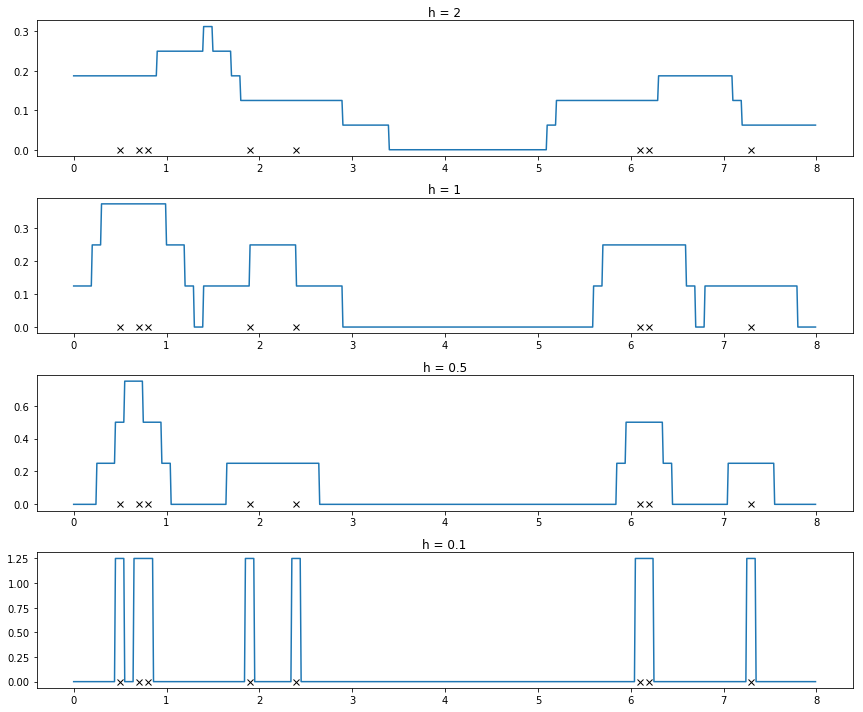
\includegraphics[height=0.9\textheight]{images/naive_estimator.png}
  \end{center}
\end{frame}

\begin{frame}[fragile]{Kernel Estimator}
A smooth weight function called a kernel to make estimate smooth. 
The most popular is the Gaussian kernel:

	\begin{equation}
		\hat p(x)=\frac{1}{Nh}\sum_{t=1}^{N}K\left( \frac{x-x^t}{h}\right)
	\end{equation}
	\begin{equation}
		K(u)=\frac{1}{2\pi}exp\left(\frac{-u^2}{2}\right)
	\end{equation}    

\end{frame}

\begin{frame}[fragile]{Kernel Estimator}
  \begin{center}
    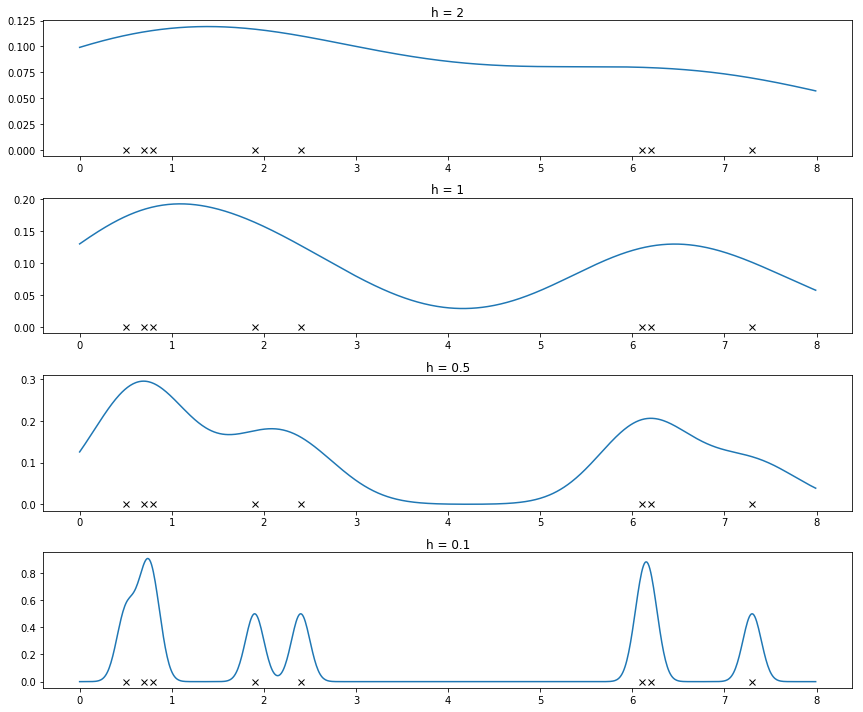
\includegraphics[height=0.9\textheight]{images/kernel_estimator.png}
  \end{center}
\end{frame}

\begin{frame}[fragile]{k-Nearest Neighbor Estimator}
The nearest neighbor class of estimators adapts the amount of smoothing
to the local density of data. The degree of smoothing is controlled by k,
the number of neighbors taken into account, which is much smaller than
N, the sample size.\\For each x:  \:  \(  d_{1}(x)\leqslant d_{2}(x)\leqslant  ...\leqslant d_{N}(x)\)\: is defined
  
 The k-nearest neighbor (k-nn) density estimate is:

	\begin{equation}
		\hat p(x)=\frac{k}{2Nd_{k}(x)}
	\end{equation}
   

\end{frame}

\begin{frame}[fragile]{k-Nearest Neighbor Estimator}
  \begin{center}
    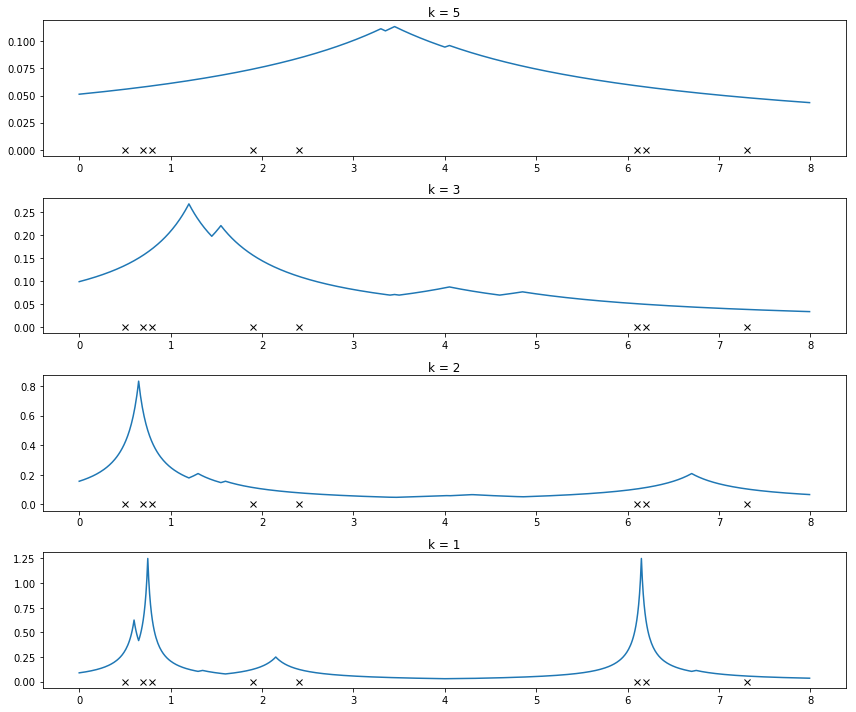
\includegraphics[height=0.9\textheight]{images/knn_estimator.png}
  \end{center}
\end{frame}


\begin{frame}[fragile]{But there are still parameters!?}
  \begin{itemize}
    \item output still depends on \textit{smoothing parameters}: kernel spread $h$ or number of neighbors $k$
    \item small parameters lead to small bias, but large variance and vice versa
    \item if the noise in the data is small, but we choose $k$ or $h$ high, we \textit{oversmooth}
    \item if the noise in the data is high, but we choose $k$ or $h$ small, we \textit{undersmooth}
    \item[$\Rightarrow$] use cross-validation to find the best parameter
  \end{itemize}
\end{frame}


\begin{frame}[fragile]{Multivariate kernel density estimator}


m-dimensional observations:\: \(X=\left(x^{t}\right)^{N}_{t=1}\)

Kernel density estimator:
	\begin{equation}
		\hat p(x)=\frac{1}{Nh^m}\sum_{t=1}^{N}K\left( \frac{x-x^t}{h}\right)
	\end{equation}
	
	\begin{equation}
		K(u)=\frac{1}{\left(2\pi\right)^{m/2}|S|^{1/2}}exp\left(-\frac{1}{2}u^{T}S^{-1}u\right)
	\end{equation} 	
\end{frame}

\begin{frame}[fragile]{Multivariate kernel density estimator}
  \begin{center}
  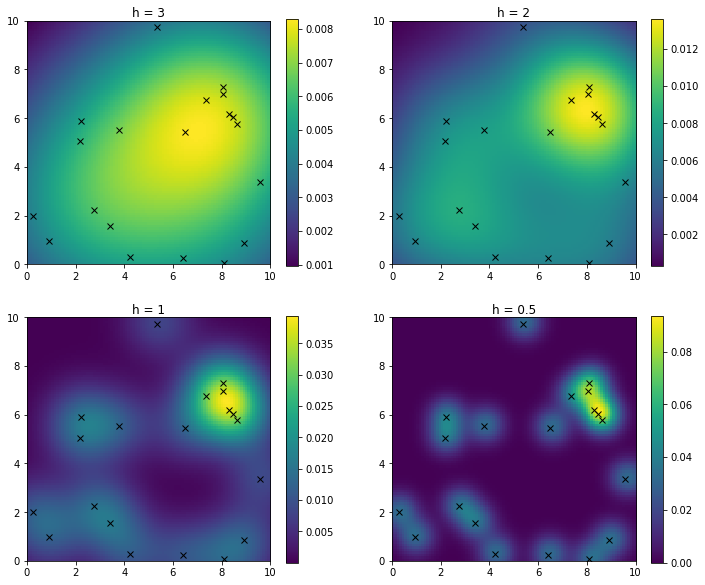
\includegraphics[height=0.9\textheight]{images/multidddd.png}
  \end{center}
\end{frame}

\section{Nonparametric Classification}
%\   
\begin{frame}[fragile]{Kernel Classification}
  

We can estimate class-conditional densities $ p(x|C_{i})$ also with a nonparametric kernel approach:
	\begin{equation}
		\hat p(x|C_{i})=\frac{1}{N_{i}h^{d}}\sum^{N}_{t=1}K\left(\frac{x-x^{t}}{h}\right)r^{t}_{i}
	\end{equation} 	

For the prior density of the classes, we have the MLE:
\begin{equation}
  \hat p(C_i) = \frac{N_i}{N} 
\end{equation}

Then classify with:
\begin{equation}
  \text{class}(x) = argmax_i \left \{\hat p(x|C_i)\hat p(C_i) \right \}
\end{equation}
		
\end{frame}	

\begin{frame}[fragile]{Kernel Classification}
\begin{center}
  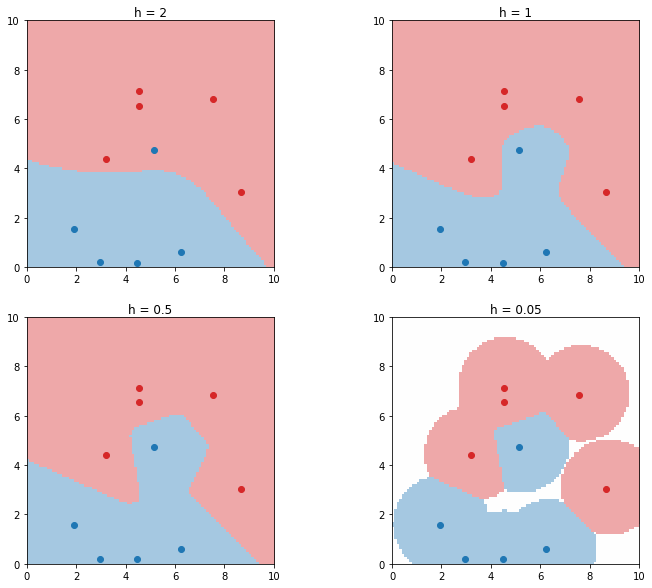
\includegraphics[height=0.9\textheight]{images/classification_kernel.png}
\end{center}
\end{frame}


\begin{frame}[fragile]{k-nn Classification}	
For the knn approach, we get the following densities:
	\begin{equation}
		\hat p(x|C_{i})=\frac{k_{i}}{N_{i}V^{k}(x)}
	\end{equation} 		
  
\begin{enumerate}[\hspace{2cm}]
  \item[$V^{k}(x)$:] the volume of the d-dimensional hypersphere centered
  at x, with radius $||x-x_{(k)}||$ where $x_{(k)}$ is the k-th nearest observation
  to x (among all neighbors from all classes of x)
  \item[$k_i$:] the number of neighbors from the $k$ nearest neighbors, that belong to class $C_i$
\end{enumerate}	
\end{frame}


\begin{frame}[fragile]{k-nn Classification}
	We can now calculate the marginal probability for the data:
  
  \begin{align}
    \hat p(x) &= \sum_i \hat p(x | C_i) \hat p(C_i)\\
              &= \sum_i \frac{k_{i}}{N_{i}V^{k}(x)} \frac{N_i}{N}\\
              &= \sum_i \frac{k_{i}}{NV^{k}(x)}\\
              &= \frac{k}{NV^{k}(x)}
  \end{align}
\end{frame}

\begin{frame}[fragile]{k-nn Classification}
	Classification is done with:
  
  \begin{align}
    \hat p(C_i | x) &= \frac{\hat p(x|C_i) \hat p(C_i)}{\hat p(x)}\\
                    &= \frac{\frac{k_{i}}{N_{i}V^{k}(x)}\frac{N_i}{N}}{\frac{k}{NV^{k}(x)}} \\
                    &= \frac{k_i}{k}
  \end{align}
  
  \begin{equation}
    \text{class}(x) = argmax_i \left \{\hat p(C_i | x) \right \}
  \end{equation}
\end{frame}

\begin{frame}[fragile]{k-nn Classification}
\begin{center}
  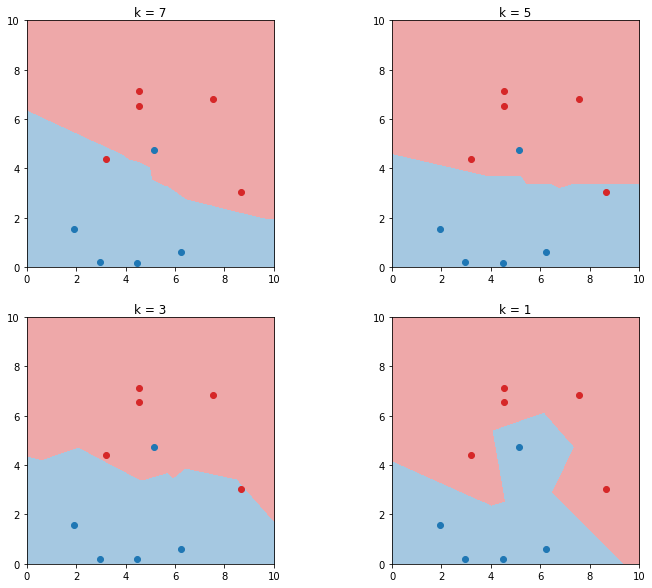
\includegraphics[height=0.9\textheight]{images/classification_knn.png}
\end{center}
\end{frame}


\begin{frame}[fragile]{Condensed Nearest Neighbor}
In order to descrease time and space complexity, the training set can be condensed. The error should not change.

\footnotesize
\begin{itemize}\setlength\itemsep{0.1em}
  \item[] Z = \{\}
  \item[] While Z still changes:
  \item[] \hspace{0.5cm} For all x $\in$ X (in random order):
  \item[] \hspace{1cm} Find z $\in$ Z which is closest to x
  \item[] \hspace{1cm} If class(x) $\ne$ class(z): add x to Z
\end{itemize}

\normalsize
The algorithm can yield quite different results, because of the randomness.
\end{frame}

\begin{frame}[fragile]{Condensed Nearest Neighbor}
\begin{center}
  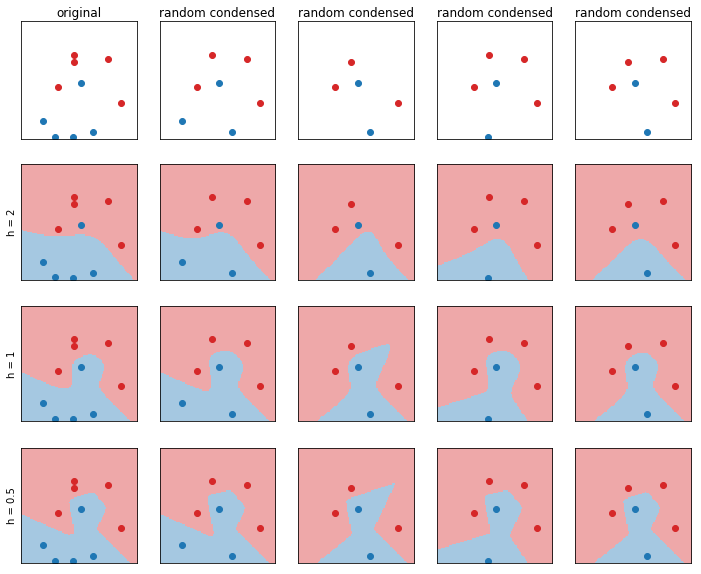
\includegraphics[height=0.9\textheight]{images/condensed_classification.png}
\end{center}
\end{frame}

\begin{frame}[fragile]{Distance-Based Classification}
Nonparametric classification relies on a \textit{distance measure} to specify, which class is the "closest".

Different distance measures make more or less sense, depending on the problem.

For parametric we had e.g. the Mahalanobis distance:
\begin{equation}
	D(x,m_i)=(x-m_i)^T S_i^{-1} (x-m_i)
\end{equation} 
\end{frame}

\begin{frame}[fragile]{Distance-Based Classification}
The main idea of nonparametric distance learning is to have a distance measure for each neighborhood, e.g. in k-nn.

Thus we need a distance measure between a point and an instance of the training set, e.g. with Mahalanobis
\begin{equation}
	D(x,x^t|M)=(x-x^t)^{T}M(x-x^t)
\end{equation} 
where M is a parameter and can be learned from the training set to optimize this measure (e.g. with the \textit{large margin nearest neighbor} algorithm).
\end{frame}


\begin{frame}[fragile]{Distance-Based Classification}
  \begin{equation}
  	D(x,x^t|M)=(x-x^t)^{T}M(x-x^t)
  \end{equation} 
  Overfitting high dimensional data can be reduced by using a low-rank approximation of M. The Mahalanobis distance for this sparce M corresponds to the (squared) euclidean distance in a subspace.
\end{frame}

\begin{frame}[fragile]{Distance-Based Classification}
  \begin{center}
    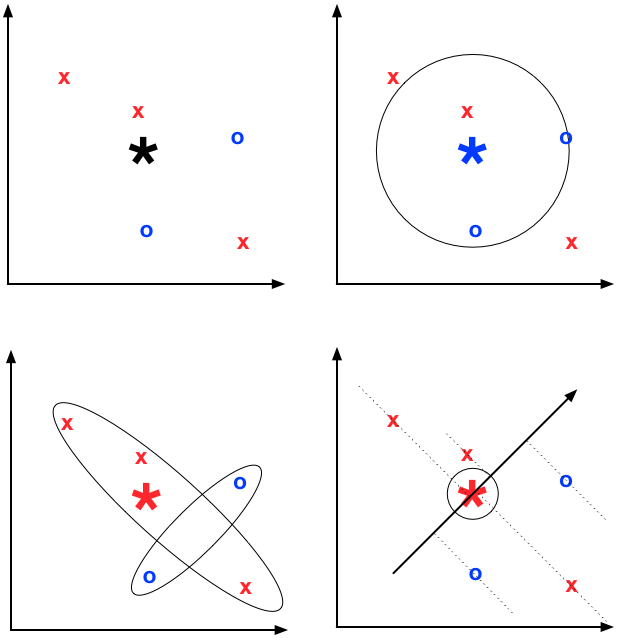
\includegraphics[height=0.9\textheight]{images/distancestuff.png}
  \end{center}
\end{frame}




\begin{frame}[fragile]{Hamming distance}
Hamming distance between two strings of equal length is the number of positions at which the corresponding symbols are different.
	\begin{equation}
		HD(x,x^t)=\sum_{j=1}^{d}1(x_j\neq x^{t}_{j})
	\end{equation} 
\end{frame}
\begin{frame}[fragile]{Outlier Detection}
Local outlier factor that comfactor pares the denseness of the neighborhood of an instance with the average
denseness of the neighborhoods of its neighbors 
\begin{equation}
LOF(x)=\frac{d_k(x)}{\sum_{s\in N(X)}d_k(s)/|N(x)|}
\end{equation} 
If LOF(x) is close to 1, x is not an outlier; as it gets larger, the probability that it is an outlier increases 
\end{frame}


\section{Nonparametric Regression}
\begin{frame}[fragile]{Nonparametric Regression: Smoothing Models}
Running Mean Smoother

\begin{equation}
g(x)=\frac{\sum_{t=1}^{N}w\left(\frac{x-x^t}{h}\right)r^t}{\sum_{t=1}^{N}w\left(\frac{x-x^t}{h}\right)}
 \qquad
w(u)=\begin{cases} 1, & \mbox{if } |u|<h \\ 0, & \mbox{otherwise } \end{cases}
\end{equation} 

Kernel Smoother
\begin{equation}
g(x)=\frac{\sum_{t=1}^{N}K\left(\frac{x-x^t}{h}\right)r^t}{\sum_{t=1}^{N}K\left(\frac{x-x^t}{h}\right)}
\end{equation} 
\end{frame}

\begin{frame}[fragile]{Nonparametric Regression: Smoothing Models}
  \begin{center}
    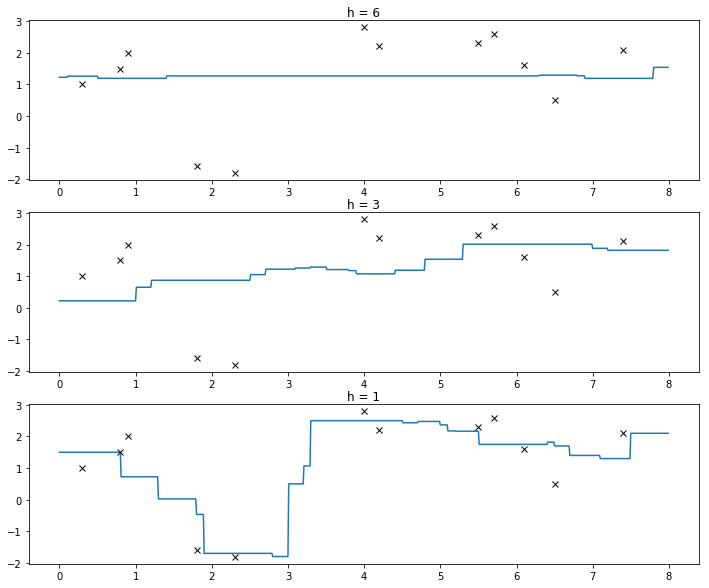
\includegraphics[height=0.9\textheight]{images/running_mean_smoother.png}
  \end{center}
\end{frame}

\begin{frame}[fragile]{Nonparametric Regression: Smoothing Models}
  \begin{center}
    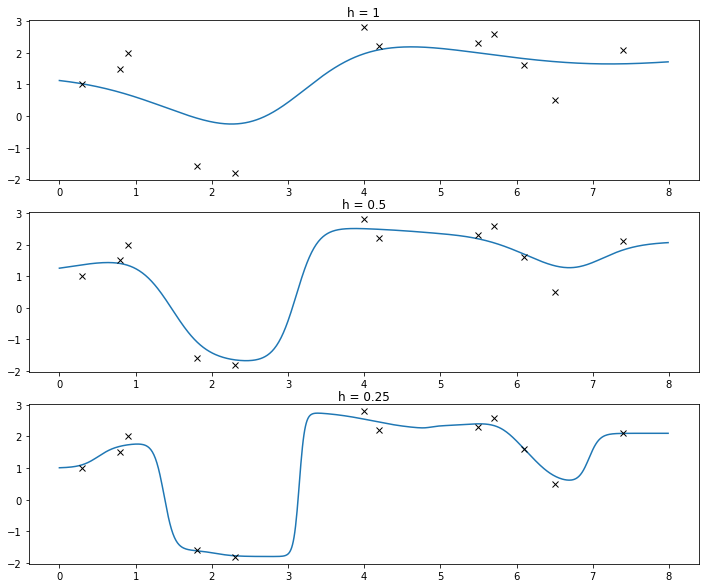
\includegraphics[height=0.9\textheight]{images/kernel_smoother.png}
  \end{center}
\end{frame}

\begin{frame}[fragile]{Nonparametric Regression: Smoothing Models}
  Running Line Smoother
  \begin{center}
    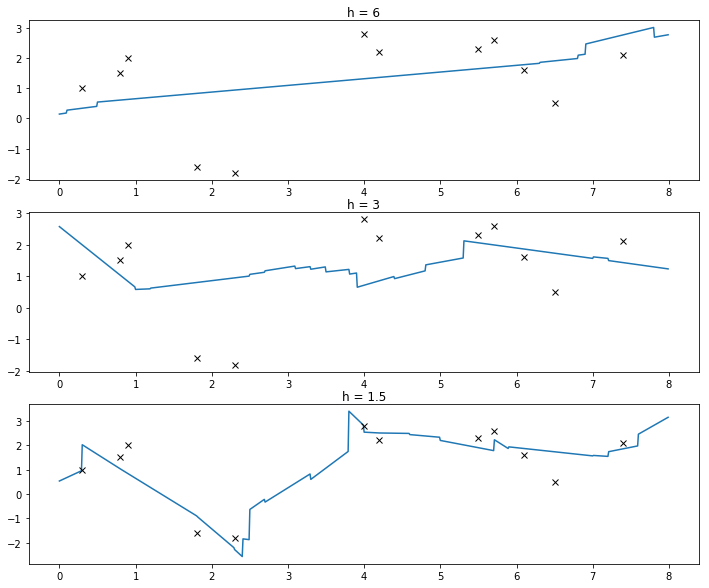
\includegraphics[height=0.8\textheight]{images/running_line_smoother.png}
  \end{center}
\end{frame}


\section{Remarks}

\begin{frame}[fragile]{Remarks}
  \begin{itemize}
    \item algorithms were proposed many years ago but were only recently used due to computational complexity
    \item for high dimensional data, the amount of needed intances increases exponentially
    \item another famous example are support vectore machines (see later presentation)
  \end{itemize}
  
\end{frame}

\end{document}